\documentclass[eng]{kjas3}
\usepackage{amsmath, natbib}
\usepackage{graphics, graphicx,multirow,subfigure,enumerate}
%\bibliographystyle{amsplain}

%% ==================================================================
%% Templete File for The Korean Journal of Applied Statistics
%% Korean Statistical Society (office@kss.or.kr)
%% ==================================================================

%\def\AMSTeX{$\cal A\kern-.1667em \lower.5ex\hbox{$\cal M$}\kern-.125em S$-\TeX}

%\submit{draft}
% ==================== Do not Modify here ============================
\submit{final}
\volumn{00}{0}{0000}
\receive{0000}{0}{0} \revise{0000}{0}{0}  \accept{0000}{0}{0}
\setpagenum{1}
% ====================================================================
% ====================================================================

\heading{The Running Title}{Author 1, Author 2, Author 3}

\begin{document}

\title{Korean Journal of Applied Statistics Style Guide\footnote{Footnote for research fund.}}

\author{
Author 1\address[a]{Department of Statistics, University of Author1;} 
Author 2\footnote{Corresponding author: Professor, 
Department of Statistics, University Author1, 
(13703) 86-1 Hankang-Dong, Mapo-Gu, Seoul, Korea, Repulic of. 
E-mail: office@kss.or.kr}\same[a]
Author 3\address[b]{Department of Statistics, University of Author3}
}

\begin{abstract}
This document explains how authors should use style file in order
to submit Korean \LaTeX{} version of their papers to 
\textit{The Korean Journal of Applied Statistics}. 
We recommend authors to follow the format here if it is not necessary. 
To use these files we assume that you have a basic \TeX{} installation (including the
necessary files to run \LaTeX{}). Along with the sample \LaTeX{}
file ({\tt sample.tex}) you should also receive {\tt kjas3.sty}. 
You may put this style file into the current
directory where you are composing the \LaTeX{} file.
\end{abstract}

\keywords{first keyword, second keyword, third keyword, fourth keyword}

%%%%%%%%%%%%%%%%%%%%%%%%%%%%%%%%%%%%%%%%%%%%%%%%%%%%%%%%%%%%%%%%%%%%%%%%%%%%%%%%%%%%%%%%%%%
%%%%%%%%%%%%%%%%%%%%%%%%%%%%%%%%%%%%%%%%%%%%%%%%%%%%%%%%%%%%%%%%%%%%%%%%%%%%%%%%%%%%%%%%%%%
%%%%%%%%%%%%%%%%%%%%%%%%%%%%%%%%%%%%%%%%%%%%%%%%%%%%%%%%%%%%%%%%%%%%%%%%%%%%%%%%%%%%%%%%%%%

\section{서론} 
이 예제화일은 한국통계학회 홈페이지의 학회지 응용통계연구(KJAS)에서
제출 논문용 스타일 화일({\tt kjas3.cls})을 다운받아 이용할 수 있다.
KJAS의 스타일 파일의 변경에 대한 가장 큰 이유는 KJAS의 편집을 위해 사용하던 한글 \LaTeX{}가 
더 이상 서비스가 되지 않기때문이다. 
이에 KJAS의 편집국에서 현재 가장 보편적으로 사용되는 MitTex이나 TexLive에서 
\LaTeX{}의 사용을 위해서이다. 
이에 한국통계학회의 또 다른 저널인 Communications for Statistical Applications and Methods (CSAM)의 스타일과 
환경을 비슷하게하여, 많은 국내 저자들에게 보다 익숙한 \LaTeX{}환경을 제공하고자 한다.
KJAS의 새로운 \LaTeX{}스타일에 대해서는 CSAM 스타일 가이드를 참고하면 더욱 쉽게 사용할 수 있을 것이다.

``{\tt csam.cls}''을 기반으로 변경되어 전에 사용되던 KJAS의 스타일과 차이는 당연히 있으며
주목할 만한 차이는 다음과 같다.
%
\begin{enumerate}
\item 접수일, 수정일, 채택일이 요약(abstract)에 따로 나오지 않고 참고문헌의 끝에 영문으로 한번 나옴

\item 한글과 영문의 폰트가 바뀜

\item 그림과 표의 번호가 장별 표기인 ``\#.\#''이 아니라 순차적으로 표기됨
\end{enumerate}
%

그리고 {\tt kjas3.cls}로 작성된 \LaTeX{}문서는 {\tt pdfLaTeX}로 컴파일 하기를 적극 추천한다.
%%%%%%%%%%%%%%%%%%%%%%%%%%%%%%%%%%%%%%%%%%%%%%%%%%%%%%%%%%%%%%%%%%%%%%%%%%%%%%%%%%%%%%%%%%%
%%%%%%%%%%%%%%%%%%%%%%%%%%%%%%%%%%%%%%%%%%%%%%%%%%%%%%%%%%%%%%%%%%%%%%%%%%%%%%%%%%%%%%%%%%%
%%%%%%%%%%%%%%%%%%%%%%%%%%%%%%%%%%%%%%%%%%%%%%%%%%%%%%%%%%%%%%%%%%%%%%%%%%%%%%%%%%%%%%%%%%%

\section{논문 작성법}
본문의 작성을 위해서는 화일의 첫 부분에 환경을 정의해야
하는데 특별한 경우를 제외하고는 본 표본화일의 내용을 그대로
따라하기를 권장한다.

논문의 작성 양식은 일반적으로 논문의 제목, 저자, 소속, 요약, 주요용어, 몇 개의 절로 이루어진 본문, 부록, 감사의 글, 참고문헌의 순서로 구성되며, 여기에 각종 수식과 표, 그림 등이 들어간다. 또한 마지막에는 논문의 국문 요약장이 삽입된다.
\LaTeX{}로 작성된 일반적인 논문의 구성은 다음과 같다.
\footnotesize
\begin{verbatim}
   \documentclass[eng]{kjas3}
   \usepackage{graphicx, natbib, amsmath}
   \usepackage{multirow, enumerate, array}

   \heading{The Running Head}{Author1, Author2}

   \begin{document}

     \author{ }
     \begin{abstract}
       .....
     \end{abstract}
     \keywords{}

     \section{}
     ... main body

     \begin{reference}
            .....
     \end{reference}
     
     \hauthor{ }
     \begin{habstract}
       .....
     \end{habstract}
     \hkeywords{}
   \end{document}
\end{verbatim}
\normalsize

이 예제에서 논문의 시작부분은 다음과 같다.

\footnotesize
\begin{verbatim}
\documentclass[eng]{kjas3}
\usepackage{amsmath, natbib}
\usepackage{graphics, graphicx,multirow,subfigure,enumerate}

\heading{The Running Title}{Author 1, Author 2, Author 3}
\begin{document}
\title{Korean Journal of Applied Statistics Style Guide\footnote{Footnote for research fund.}}
\author{
Author 1\address[a]{Department of Statistics, University of Author1;} 
Author 2\footnote{Corresponding author: Professor, Department of Statistics, University Author1, 
(13703) 86-1 Hankang-Dong, Mapo-Gu, Seoul, Korea, Repulic of. 
E-mail: office@kss.or.kr}\same[a]
Author 3\address[b]{Department of Statistics, University of Author3}
}
\begin{abstract}
This document explains how authors should use style file in order
to submit Korean \LaTeX{} version of their papers to 
\textit{The Korean Journal of Applied Statistics}. 
We recommend authors to follow the format here if it is not necessary. 
To use these files we assume that you have a basic \TeX{} installation (including the
necessary files to run \LaTeX{}). Along with the sample \LaTeX{}
file ({\tt sample.tex}) you should also receive {\tt kjas3.sty}. 
You may put this style file into the current
directory where you are composing the \LaTeX{} file.
\end{abstract}
\keywords{first keyword, second keyword, third keyword, fourth keyword}
\end{verbatim}
\normalsize

%%%%%%%%%%%%%%%%%%%%%%%%%%%%%%%%%%%%%%%%%%%%%%%%%%%%%%%%%%%%%%%%%%%%%%%%%%%%%%%%%%%%%%%%%%%
%%%%%%%%%%%%%%%%%%%%%%%%%%%%%%%%%%%%%%%%%%%%%%%%%%%%%%%%%%%%%%%%%%%%%%%%%%%%%%%%%%%%%%%%%%%
%%%%%%%%%%%%%%%%%%%%%%%%%%%%%%%%%%%%%%%%%%%%%%%%%%%%%%%%%%%%%%%%%%%%%%%%%%%%%%%%%%%%%%%%%%%

\section{제목, 저자 및 요약문}
논문의 서두부에는 영문으로 제목과 저자 이름, 저자의 소속 기관, 연구비 지원여부, 요약문 및 주요용어가 포함된다.
아래에 제시한 예시에 따라서 서두부를 작성하면 된다.

%%%%%%%%%%%%%%%%%%%%%%%%%%%%%%%%%%%%%%%%%%%%%%%%%%%%%%%%%%%%%%%%%%%%%%%%%%%%%%%%%%%%%%%%%%%
\subsection{절, 소절}
본문은 몇개의 절로 구성되며, 각 절은 또 몇 개의 소절로 구성될 수 있다. 응용통계연구는 절의 단위를 section, subsection, subsubsection으로 구분한다. 절의 시작은  {\verb"\section{제목}"} 으로 시작된다.

%%%%%%%%%%%%%%%%%%%%%%%%%%%%%%%%%%%%%%%%%%%%%%%%%%%%%%%%%%%%%%%%%%%%%%%%%%%%%%%%%%%%%%%%%%%
\subsection{수식 }
응용통계연구에서 수식은 \texttt{align} 환경을 사용하여 작성한다. 수식 번호는 (1.1), (1.2) 순서로 자동 부여되고
수식은 \& 기호에 맞춰서 정렬된다. 식 번호를 원하지 않는 경우는 \verb"\nonumber"를 넣거나 \texttt{align*} 환경에서 수식을 작성하면 된다. \texttt{align} 환경에서 \verb"\nonumber"를 사용하여 작성된 수식의 예시와 그 출력 결과는 아래와 같다.
\begin{verbatim}
   \begin{align}
   x^{2} + y^{2} &= z^{2}, \nonumber \\
   x^{3} + y^{3} &< z^{3}.
   \end{align}
\end{verbatim}
\begin{align}
x^{2} + y^{2} &= z^{2}, \nonumber \\
x^{3} + y^{3} &< z^{3}. \label{eq21}
\end{align}
\verb"\nonumber"가 쓰여진 줄에는 식번호가 나타나지 않는다.  \texttt{align*} 환경에서 작성한 아래의 수식에는 식번호가 나오지 않는다.
\begin{align*}
x^{2} + y^{2} &= z^{2}, \\
x^{3} + y^{3} &< z^{3}.
\end{align*}

%%%%%%%%%%%%%%%%%%%%%%%%%%%%%%%%%%%%%%%%%%%%%%%%%%%%%%%%%%%%%%%%%%%%%%%%%%%%%%%%%%%%%%%%%%%
\subsection{정리, 증명, 정의 등}
응용통계연구 한글용 스타일 화일에서는 정리, 증명, 정의, 예제 등을 위한
환경이 정의되어 있으면 이와 같은 환경은 \verb"\begin{환경이름}"으로 시작되어 \verb"\end{환경이름}"으로 끝난다. 대응되는 환경이름은
각각 theorem, proof, definition, example이다.

\begin{theorem}\label{thm1}
정리는 장 내에서 일련번호가 붙는다.
\end{theorem}
\begin{proof}
증명을 위한 proof 환경이 있으며, 증명의 끝부분에는 자동적으로 `$\square$'가 붙는다.
\end{proof}
\begin{definition}
정의를 여기에 입력한다.
\end{definition}
\begin{example}
예제를 여기에 입력한다.
\end{example}

%%%%%%%%%%%%%%%%%%%%%%%%%%%%%%%%%%%%%%%%%%%%%%%%%%%%%%%%%%%%%%%%%%%%%%%%%%%%%%%%%%%%%%%%%%%
%%%%%%%%%%%%%%%%%%%%%%%%%%%%%%%%%%%%%%%%%%%%%%%%%%%%%%%%%%%%%%%%%%%%%%%%%%%%%%%%%%%%%%%%%%%
%%%%%%%%%%%%%%%%%%%%%%%%%%%%%%%%%%%%%%%%%%%%%%%%%%%%%%%%%%%%%%%%%%%%%%%%%%%%%%%%%%%%%%%%%%%
\section{그림과 표 본문 삽입}
\subsection{그림 삽입}
응용통계연구에서 표와 그림의 삽입을 위하여 각각 \verb"figure"와  \verb"table" 환경을 사용한다.
 그림과 표의 위치는 \verb"t"(페이지 위쪽), \verb"b"(페이지 아래쪽), \verb"h"(지정된 위치)를 
 사용하여 정할 수 있는데 응용통계연구는 각 페이지 위쪽에 위치하는 것을 원칙으로 하고 있다.
그림과 표는 제목을 비롯해서 모두 영문으로 작성해야 하며 \verb"\caption{제목}"을 사용해 번호를 자동으로 부여한다.

우선 그림 작성의 예시를 살펴보기로 한다. \verb"\subfigure"를 사용하여 그림마다 제목을 넣을 수도 있다.
그림 \ref{fig:eps}는 eps파일을 입력하는 예제이고, 그림 \ref{png:jpg}은 png나 jpg파일을 삽입하는 예제이다.
여기서는 \verb"graphics"와 \verb"graphicx" 패키지에서 사용되는 \verb"\includegraphics"을 사용했지만, 
\verb"epsfig" 패키지에서 사용되는 \verb"\psfig" 명령어도 \verb"epsfig"이 선언되면 당연히 사용이 가능하다.

\begin{verbatim}
\begin{figure}[t]
  \centering
  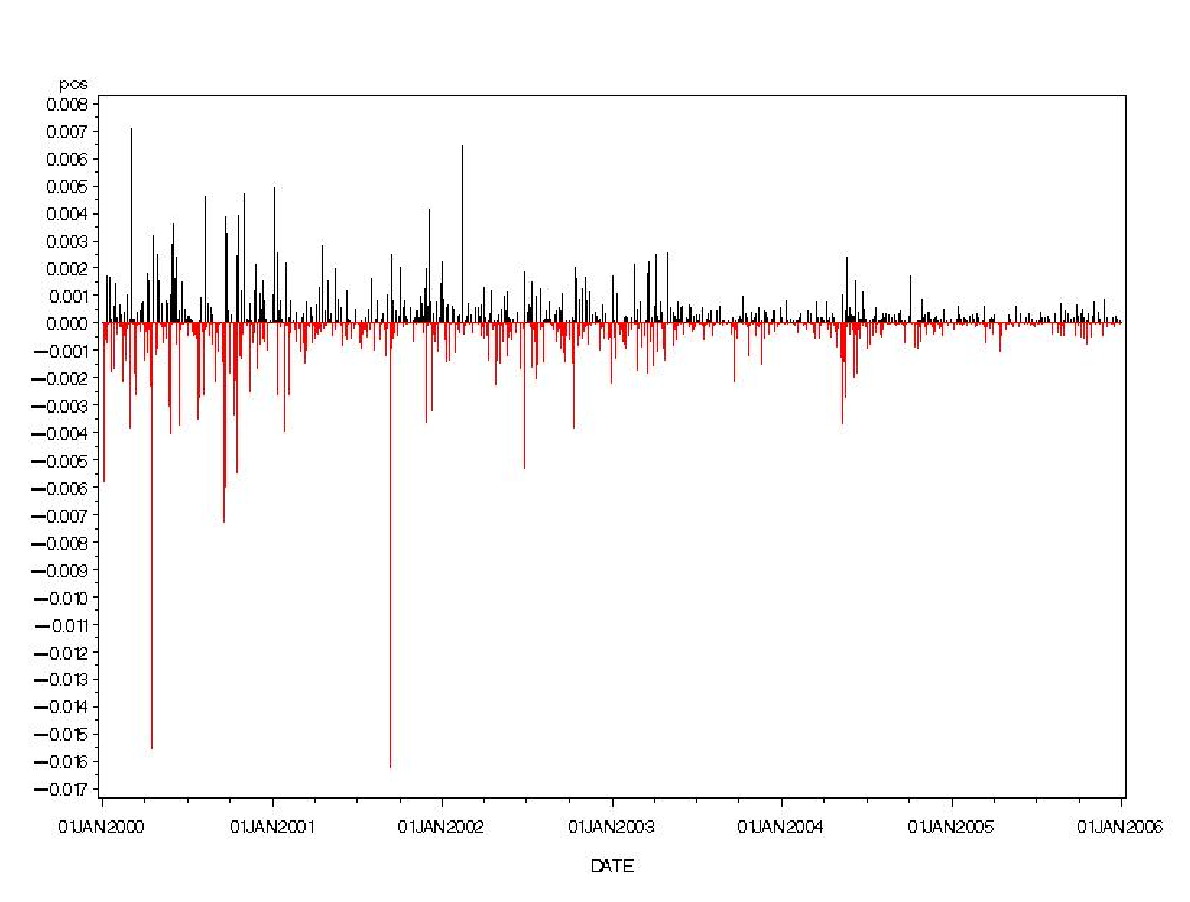
\includegraphics[height=4cm,keepaspectratio=true]{fig1.eps}
  \subfigure[subfigure title 1]{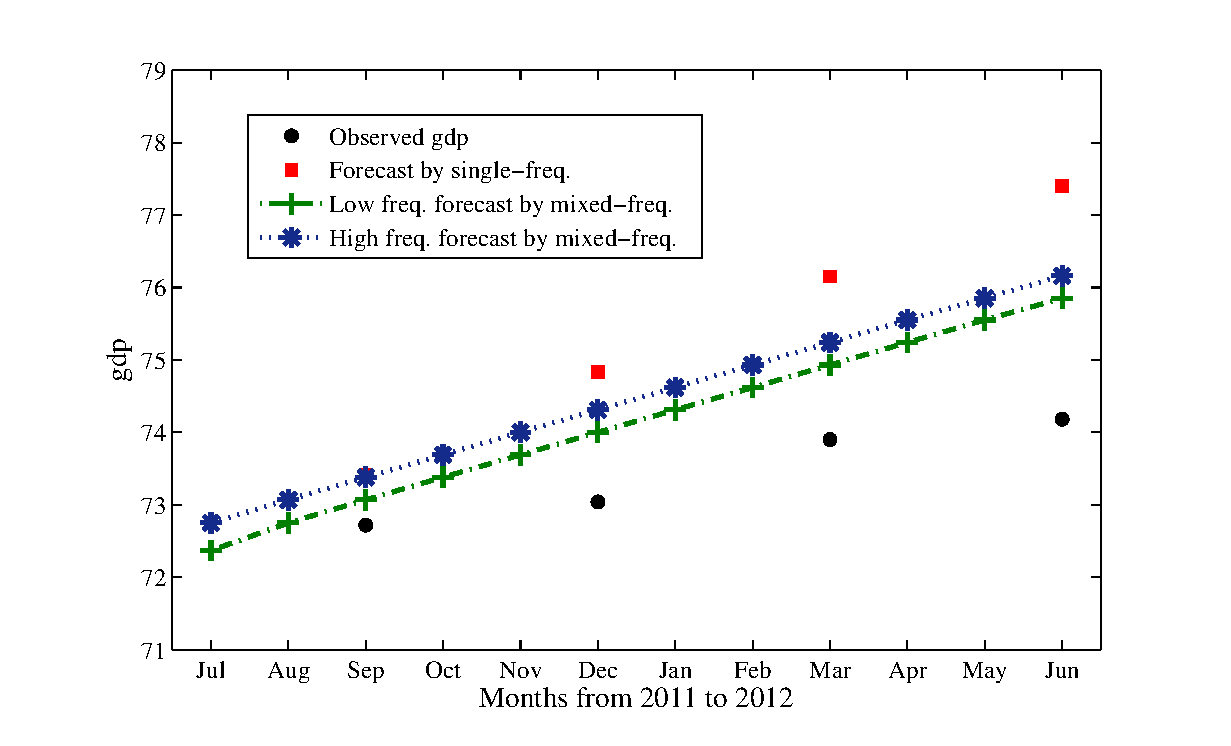
\includegraphics[width=4cm,height=4cm]{fig2.eps}}
  \subfigure[subfigure title 2]{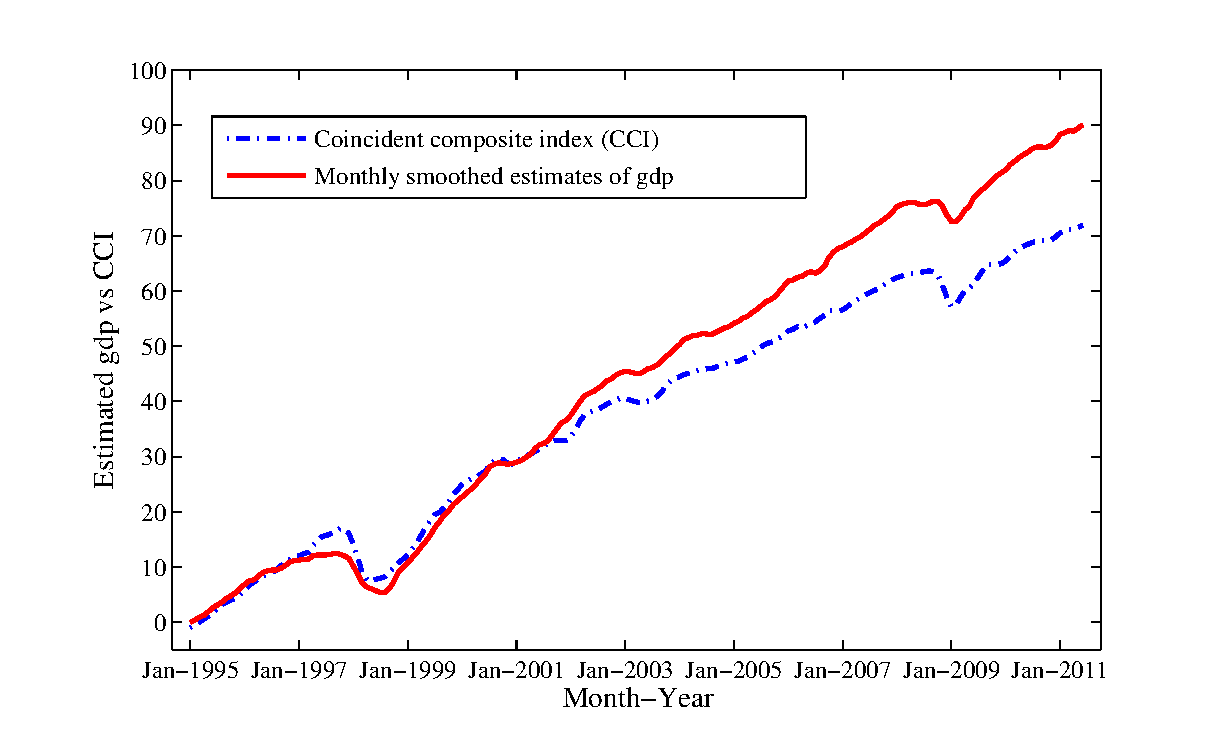
\includegraphics[width=4cm,height=4cm]{fig3.eps}}
\caption{Sample figure title} \label{fig:eps}
\end{figure}

\begin{figure}[t]
  \centering
  \subfigure[KJAS-PNG]{\includegraphics[width=7cm,height=5cm]{kjas.png}}
  \subfigure[KJAS-JPG]{\includegraphics[width=7cm,height=5cm]{kjas.jpg}}
\caption{Example for PNG and JPG files} \label{png:jpg}
\end{figure}
\end{verbatim}

\begin{figure}[t]
\centering
  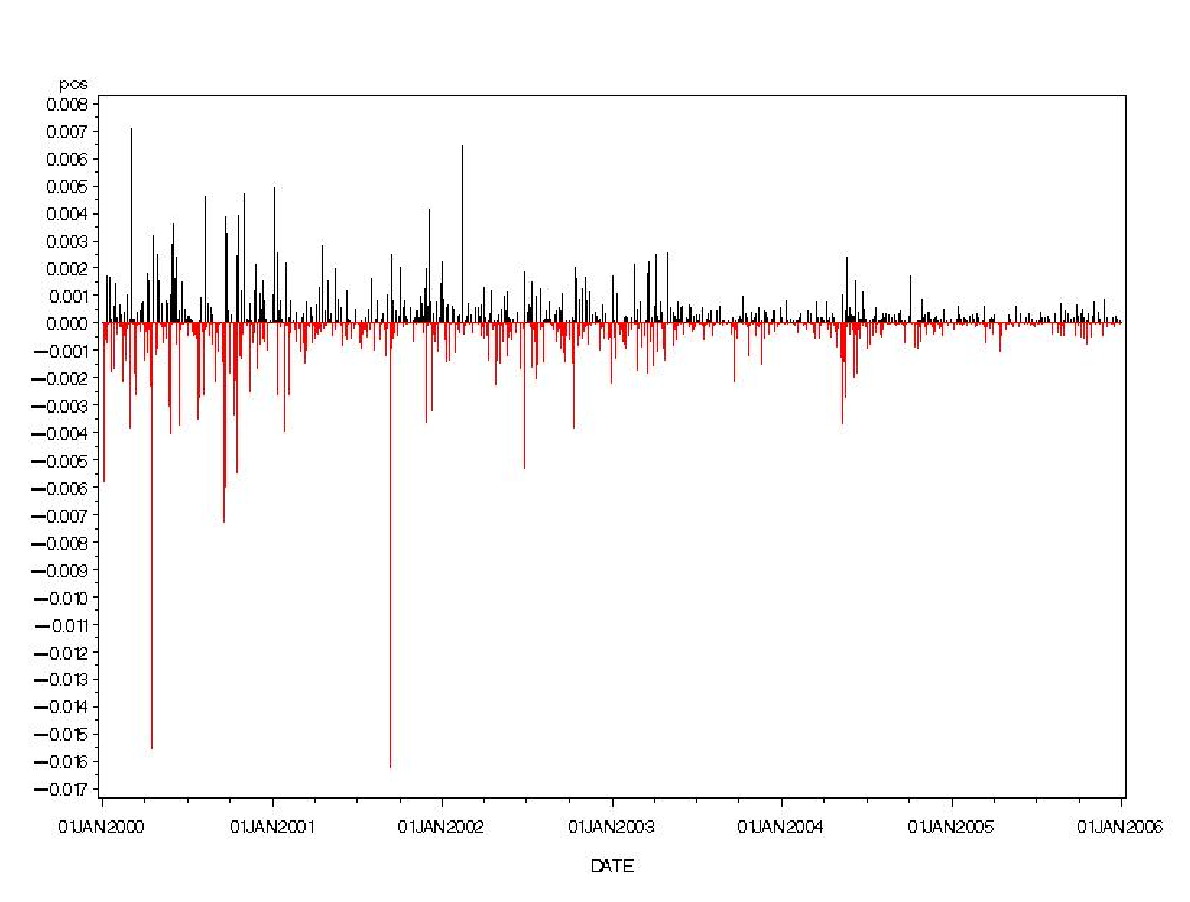
\includegraphics[width=10cm,height=4.5cm]{fig1.eps}
  \subfigure[subfigure title 1]{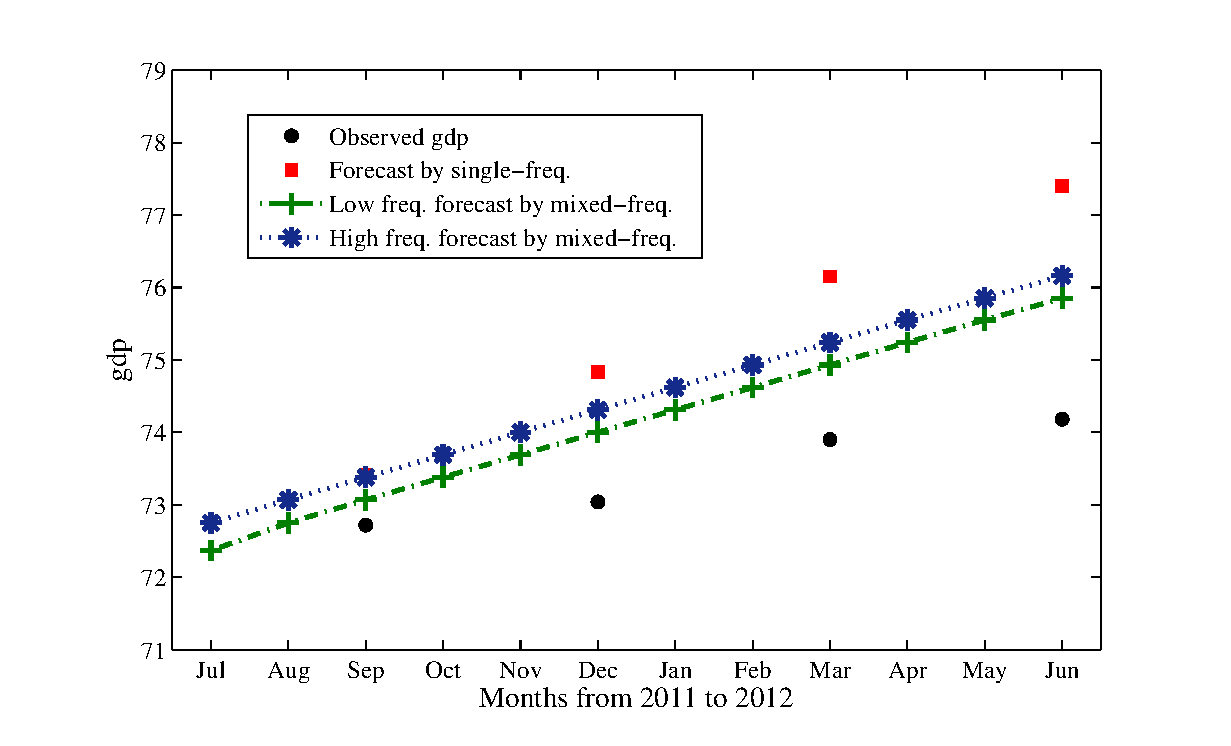
\includegraphics[width=4.3cm,height=4.3cm]{fig2.eps}}
  \subfigure[subfigure title 2]{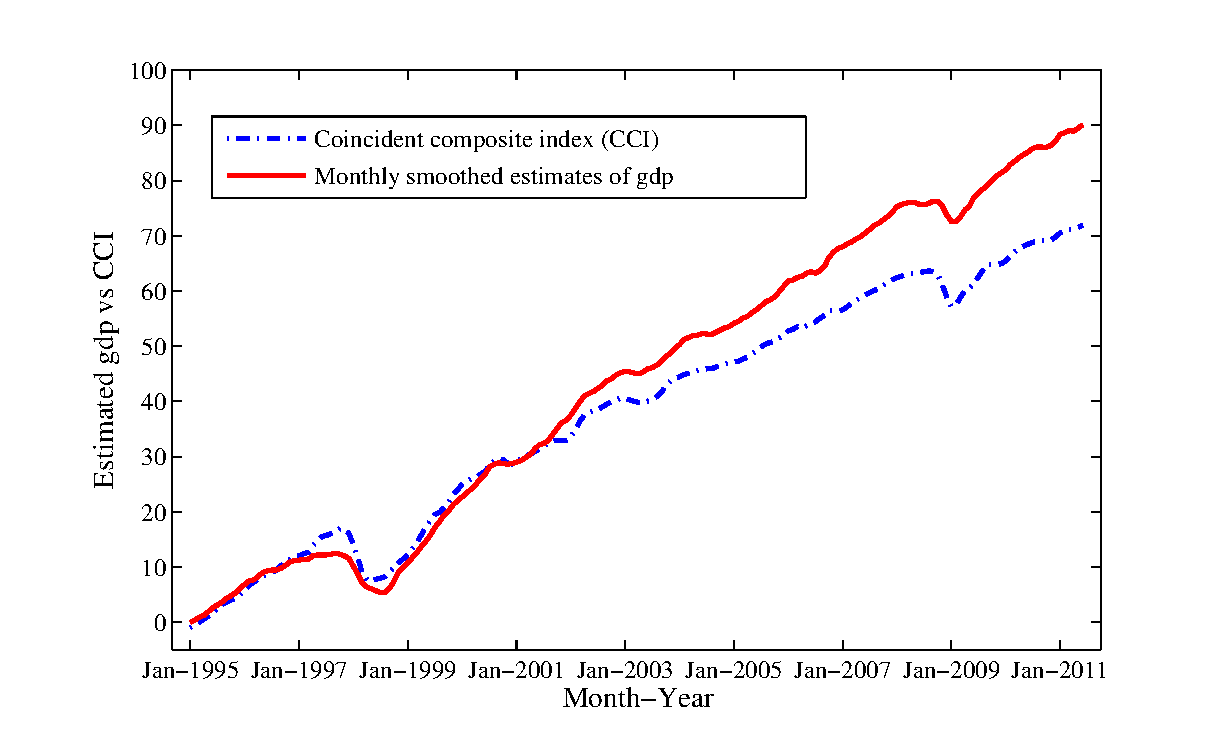
\includegraphics[width=4.3cm,height=4.3cm]{fig3.eps}}
\caption{Sample figure title}\label{fig:eps}
\end{figure}

\begin{figure}[t]
\centering
  \subfigure[KJAS-PNG]{\includegraphics[width=7cm,height=5cm]{kjas.png}}
  \subfigure[KJAS-JPG]{\includegraphics[width=7cm,height=5cm]{kjas.jpg}}
\caption{Example for PNG and JPG files} \label{png:jpg}
\end{figure}
%%%%%%%%%%%%%%%%%%%%%%%%%%%%%%%%%%%%%%%%%%%%%%%%%%%%%%%%%%%%%%%%%%%%%%%%%%%%%%%%%%%%%%%%%%%

\subsection{표 삽입}
표의 경우를 살펴보면 표의 폭을 문서의 폭 만큼의 크기로 출력해야 하며 \verb"\tabcolseq=30pt"와 같은 명령으로 적절히 조절하여 문서의 폭과 같은 넓이로 작성 할 수 있다. 또한 \verb"\multicolumn"과 \verb"\multirow"를 사용하여 여러 열과 행을 합쳐서 사용할 수 있다. 다음은 표에 대한 예시이다.
\begin{verbatim}
   \begin{table}[t]
   \caption{Structure of data.}\label{tb:data1}
   \footnotesize
   \centering
   {\tabcolsep=33.7pt
   \begin{tabular}{ccccc}
   \hline
   \multirow{2}*{$N$} & \multicolumn{4}{c}{factor level} \\\cline{2-5}
    & 1 & 2 & $\cdots$ & $I$ \\\hline
   1        & $x_{11}$ & $x_{21}$ & $\cdots$ & $x_{I1}$ \\
   2        & $x_{12}$ & $x_{22}$ & $\cdots$ & $x_{I2}$ \\
   $\vdots$ & $\vdots$ & $\vdots$ & $\ddots$ & $\vdots$ \\
   $n$      & $x_{1n}$ & $x_{2n}$ & $\cdots$ & $x_{In}$ \\
   \hline
   \end{tabular}}
   \end{table}
\end{verbatim}

\begin{table}[t]
\caption{Structure of data.} \label{tb1}
\footnotesize
   \centering
{\tabcolsep=33.7pt
\begin{tabular}{ccccc}
\hline
\multirow{2}*{$N$} & \multicolumn{4}{c}{factor level} \\\cline{2-5}
 & 1 & 2 & $\cdots$ & $I$ \\\hline
1        & $x_{11}$ & $x_{21}$ & $\cdots$ & $x_{I1}$ \\
2        & $x_{12}$ & $x_{22}$ & $\cdots$ & $x_{I2}$ \\
$\vdots$ & $\vdots$ & $\vdots$ & $\ddots$ & $\vdots$ \\
$n$      & $x_{1n}$ & $x_{2n}$ & $\cdots$ & $x_{In}$ \\
\hline
\end{tabular}}
\end{table}

%%%%%%%%%%%%%%%%%%%%%%%%%%%%%%%%%%%%%%%%%%%%%%%%%%%%%%%%%%%%%%%%%%%%%%%%%%%%%%%%%%%%%%%%%%%
%%%%%%%%%%%%%%%%%%%%%%%%%%%%%%%%%%%%%%%%%%%%%%%%%%%%%%%%%%%%%%%%%%%%%%%%%%%%%%%%%%%%%%%%%%%
%%%%%%%%%%%%%%%%%%%%%%%%%%%%%%%%%%%%%%%%%%%%%%%%%%%%%%%%%%%%%%%%%%%%%%%%%%%%%%%%%%%%%%%%%%%
\section{수식, 표, 그림 등에 대해 라벨 (label)기능 사용하기}
\verb"\label" 명령은 번호를 저장하였다가 \verb"\ref"를 이용하여 번호를 호출할때 사용된다. 
이러한 기능은 수식, 그림, 표, 절, 정리, 정의, 보조정리, 예제 등에 두루 사용할 수 있다. 
\verb"\label{thm1}"이 붙혀진 정리에 대한 인용은 ``정리 1.1''과 같이 직접 기입하는 대신
 ``정리 \verb"\ref{thm1}"''과 같이 쓸 수 있다. 수식의 경우,  식  (\verb"\ref{eq21}")로 기입하는데 
\verb"\eqref{eq21}"를 사용하면 ( )를 따로 쓰는 번거로움을 줄일 수 있다. 
이러한 기능을 이용하면 논문 작성 시, 수식 등의 추가로 수식번호가 바뀌더라도 
인용문은 수정하지 않아도 되어 매우 편리한 기능이라고 할 수 있다. 
그러나 한글 논문의 경우 번호가 바뀌면 조사가 달라질 수 있으므로 조사에 대해 유의하여야 한다.
다음은 \verb"\label"의 예시들이다.
\begin{verbatim}
   식  \begin{align}
       a + b = c    \label{eq1}
       \end{align}
   절  \section{title}\label{sec1}
   그림  \cation{title}\label{fig1}
   정의  \begin{definition}\label{def1}
\end{verbatim}

여러개의 항목을 나열 한때는 \verb"enumerate", \verb"itemize", \verb"description" 환경을 사용할 수 있다. 그리고 각각의 항목들은 \verb"\item"이라는 명령어로 시작해야 한다. \verb"enumerate"의 경우는 자동으로 레이블을 순서대로 넣어준다 물론 \verb"\item[레이블]"로 직접 레이블을 넣어줄 수도 있다.
\begin{verbatim}
   \begin{enumerate}[레이블]           \begin{enumerate}
   \item 나열하고자 하는 항목1             \item[레이블] 나열하고자 하는 항목1
   \item 나열하고자 하는 항목2             \item[레이블] 나열하고자 하는 항목2
   \end{enumerate}                    \end{enumerate}
\end{verbatim}

%\begin{enumerate}[Step 1]
% \item 나열하고자 하는 항목1
% \item 나열하고자 하는 항목2
% \item 나열하고자 하는 항목3
%\end{enumerate}

%%%%%%%%%%%%%%%%%%%%%%%%%%%%%%%%%%%%%%%%%%%%%%%%%%%%%%%%%%%%%%%%%%%%%%%%%%%%%%%%%%%%%%%%%%%
%%%%%%%%%%%%%%%%%%%%%%%%%%%%%%%%%%%%%%%%%%%%%%%%%%%%%%%%%%%%%%%%%%%%%%%%%%%%%%%%%%%%%%%%%%%
%%%%%%%%%%%%%%%%%%%%%%%%%%%%%%%%%%%%%%%%%%%%%%%%%%%%%%%%%%%%%%%%%%%%%%%%%%%%%%%%%%%%%%%%%%%
\section{참고문헌}
참고문헌을 작성할 때에는 전부 영어로 작성해야 하며 문헌이 저서인 경우와 논문인 경우에 따라 작성 형식이 달라진다. 
만약 저서라면 저서명을 이탤릭으로, 논문이라면 학술지명을 이탤릭으로 표시한다. 다음은 참고문헌의 예시이다.
그리고 참고문헌 끝에 논문의 접수일, 재투고일 그리고 채택일이 자동적으로 등장한다.
본 샘플에서의 참고문헌은 다음의 명령어로 작성되어 졌다.
\begin{verbatim}
\begin{reference}
\item[] Box, G. E. P. and Draper, N. R. (1969). {\em Evolutionary Operation},
        John Wiley \& Sons, New York.
\item[] Wald, A. (1949). Note on the consistency of the maximum likelihood
        estimate, {\em Annals of Mathematical Statistics}, {\bf 20}, 595--601.
\item[] Seking, J. W. (2005). Forecasting item production with ARIMA model,
        {\em Technical Paper}, Available from: http://tech.journal.net/2005/
        05102.pdf
\end{reference}
\end{verbatim}
%%%%%%%%%%%%%%%%%%%%%%%%%%%%%%%%%%%%%%%%%%%%%%%%%%%%%%%%%%%%%%%%%%%%%%%%%%%%%%%%%%%%%%%%%%%
%%%%%%%%%%%%%%%%%%%%%%%%%%%%%%%%%%%%%%%%%%%%%%%%%%%%%%%%%%%%%%%%%%%%%%%%%%%%%%%%%%%%%%%%%%%
%%%%%%%%%%%%%%%%%%%%%%%%%%%%%%%%%%%%%%%%%%%%%%%%%%%%%%%%%%%%%%%%%%%%%%%%%%%%%%%%%%%%%%%%%%%

{\appendix \section*{}
논문에 부록이 필요한 경우 다음과 같은 형식을 사용하면 된다. 
첫째 부록에 특별한 제목이 없는 경우에는 \verb"\section*{}"과 같이 쓰고 부록의 내용을 입력한다. 
부록에 제목이 있다면 \verb"\section*{부록제목}" 을 넣은 뒤 사용하면 된다. 
셋째 부록이 둘 이상이라면 \verb"\section{부록제목}"의 형식을 따른다.
참고로 부록 내의 수식이나 표, 그림의 번호에는 영문자가 붙는다.
 즉 수식 번호는 (A.1)과 같은 형식으로 부여된다.

\begin{table}[t]
\caption{Structure of data.} \label{tb1}
\footnotesize
   \centering
{\tabcolsep=33.7pt
\begin{tabular}{ccccc}
\hline
\multirow{2}*{$N$} & \multicolumn{4}{c}{factor level} \\\cline{2-5}
 & 1 & 2 & $\cdots$ & $I$ \\\hline
1        & $x_{11}$ & $x_{21}$ & $\cdots$ & $x_{I1}$ \\
2        & $x_{12}$ & $x_{22}$ & $\cdots$ & $x_{I2}$ \\
$\vdots$ & $\vdots$ & $\vdots$ & $\ddots$ & $\vdots$ \\
$n$      & $x_{1n}$ & $x_{2n}$ & $\cdots$ & $x_{In}$ \\
\hline
\end{tabular}}
\end{table}
}
%%%%%%%%%%%%%%%%%%%%%%%%%%%%%%%%%%%%%%%%%%%%%%%%%%%%%%%%%%%%%%%%%%%%%%%%%%%%%%%%%%%%%%%%%%%
%%%%%%%%%%%%%%%%%%%%%%%%%%%%%%%%%%%%%%%%%%%%%%%%%%%%%%%%%%%%%%%%%%%%%%%%%%%%%%%%%%%%%%%%%%%
%%%%%%%%%%%%%%%%%%%%%%%%%%%%%%%%%%%%%%%%%%%%%%%%%%%%%%%%%%%%%%%%%%%%%%%%%%%%%%%%%%%%%%%%%%%
\section*{감사의 글}
감사의 글이 필요한 경우 감사의 글에 대한 내용을 \verb"\section*{감사의 글}"로 시작하여 작성한다.


%%%%%%%%%%%%%%%%%%%%%%%%%%%%%%%%%%%%%%%%%%%%%%%%%%%%%%%%%%%%%%%%%%%%%%%%%%%%%%%%%%%%%%%%%%%
%%%%%%%%%%%%%%%%%%%%%%%%%%%%%%%%%%%%%%%%%%%%%%%%%%%%%%%%%%%%%%%%%%%%%%%%%%%%%%%%%%%%%%%%%%%
%%%%%%%%%%%%%%%%%%%%%%%%%%%%%%%%%%%%%%%%%%%%%%%%%%%%%%%%%%%%%%%%%%%%%%%%%%%%%%%%%%%%%%%%%%%
\section{국문 요약}
응용통계연구에 투고되는 논문의 마지막 페이지에는 반드시 국문 요약이 작성되어져야 한다.
페이지 마지막장에는 국문제목, 저자이름, 저자소속, 국문요약, 주요용어를 한글로 작성하여야 한다.
이를 위한 \LaTeX{}명령어는 서두에 영문으로 작성된 국문제목, 저자이름, 저자소속, 국문요약, 주요용어와 다름에
유의하여야 한다.
반드시 \verb"\htitle{}", \verb"\hauthor{}", \verb"\begin{habstract}...\end{habstract}"와 
\verb"\hkeywords{}"를 사용해야 한다.
본문 샘플에서 사용한 예제는 다음과 같다.
\begin{verbatim}
\htitle{응용통계연구 \LaTeX{}스타일 파일 가이드\footnote{연구비에 대한 기술.}}

\hauthor{
저자1\address[a]{저자 1의 소속;}
저자2\footnote{교신저자: 교수, 한국대학고 통계학과}\same[a]
저자3\address[b]{저자 3의 소속}
}

\begin{habstract}
국문요약을 여기에 작성하시면 됩니다. 
\end{habstract}

\hkeywords{용어1, 용어2, 용어3, 용어4}
\end{verbatim}

%%%%%%%%%%%%%%%%%%%%%%%%%%%%%%%%%%%%%%%%%%%%%%%%%%%%%%%%%%%%%%%%%%%%%%%%%%%%%%%%%%%%%%%%%%%
%%%%%%%%%%%%%%%%%%%%%%%%%%%%%%%%%%%%%%%%%%%%%%%%%%%%%%%%%%%%%%%%%%%%%%%%%%%%%%%%%%%%%%%%%%%
%%%%%%%%%%%%%%%%%%%%%%%%%%%%%%%%%%%%%%%%%%%%%%%%%%%%%%%%%%%%%%%%%%%%%%%%%%%%%%%%%%%%%%%%%%%
\begin{reference}
\item[] Box, G. E. P. and Draper, N. R. (1969). 
        \textit{ Evolutionary Operation}, John Wiley \& Sons, New York.
        
\item[] Wald, A. (1949). 
        Note on the consistency of the maximum likelihood estimate, 
        \textit{Annals of Mathematical Statistics}, \textbf{20}, 595--601.
        
\item[] Seking, J. W. (2005). Forecasting item production with ARIMA model,
        \textit{Technical Paper}, Available from: \texttt{http:// tech.journal.net/2005/05102.pdf}
        
\end{reference}

%%%%%%%%%%%%%%%%%%%%%%%%%%%%%%%%%%%%%%%%%%%%%%%%%%%%%%%%%%%%%%%%%%%%%%%%%%%%%%%%%%
%%%%%%%%%%%%%%%%%%%%%%%%%%%%%%%%%%%%%%%%%%%%%%%%%%%%%%%%%%%%%%%%%%%%%%%%%%%%%%%%%%
\htitle{응용통계연구 \LaTeX{}스타일 파일 가이드\footnote{연구비에 대한 기술.}}

\hauthor{
저자1\address[a]{저자 1의 소속}
저자2\footnote{교신저자: 교수, 한국대학고 통계학과}\same[a]
저자3\address[b]{저자 3의 소속}
}

\begin{habstract}
국문요약을 여기에 작성하시면 됩니다. 
\end{habstract}

\hkeywords{용어1, 용어2, 용어3, 용어4}

\end{document}
